\section{Example: Selecting a Magnetic Field Model}

%\vspace{-1cm}

After

~~~~~\senv

our starting point is \wee. We copy it to \wie:

~~~~~\gtis{cp \$WAVE/input/wave.example wave.in}

and enter

~~~~~\WSH

The GUI pops up, select in the upper menu bar \scap{Comment} and
to change the user title

~~~~~\scap{WAVE.EXAMPLE}

to

~~~~~\gtis{Planar Undulator}

Hit \scap{OK} to leave the widget. Select \gtise{Sel. Mag.}.

A menu pops up:

\begin{itemize} \renewcommand\labelitemi{--}
\item
Click

\witem{Elliptical undulator (analytical model)}

to deselect the current model and

\witem{Halbach undulator/wiggler with end poles}

to select the planar undulator model.
\end{itemize}

\begin{figure}[htb]
    \centering
    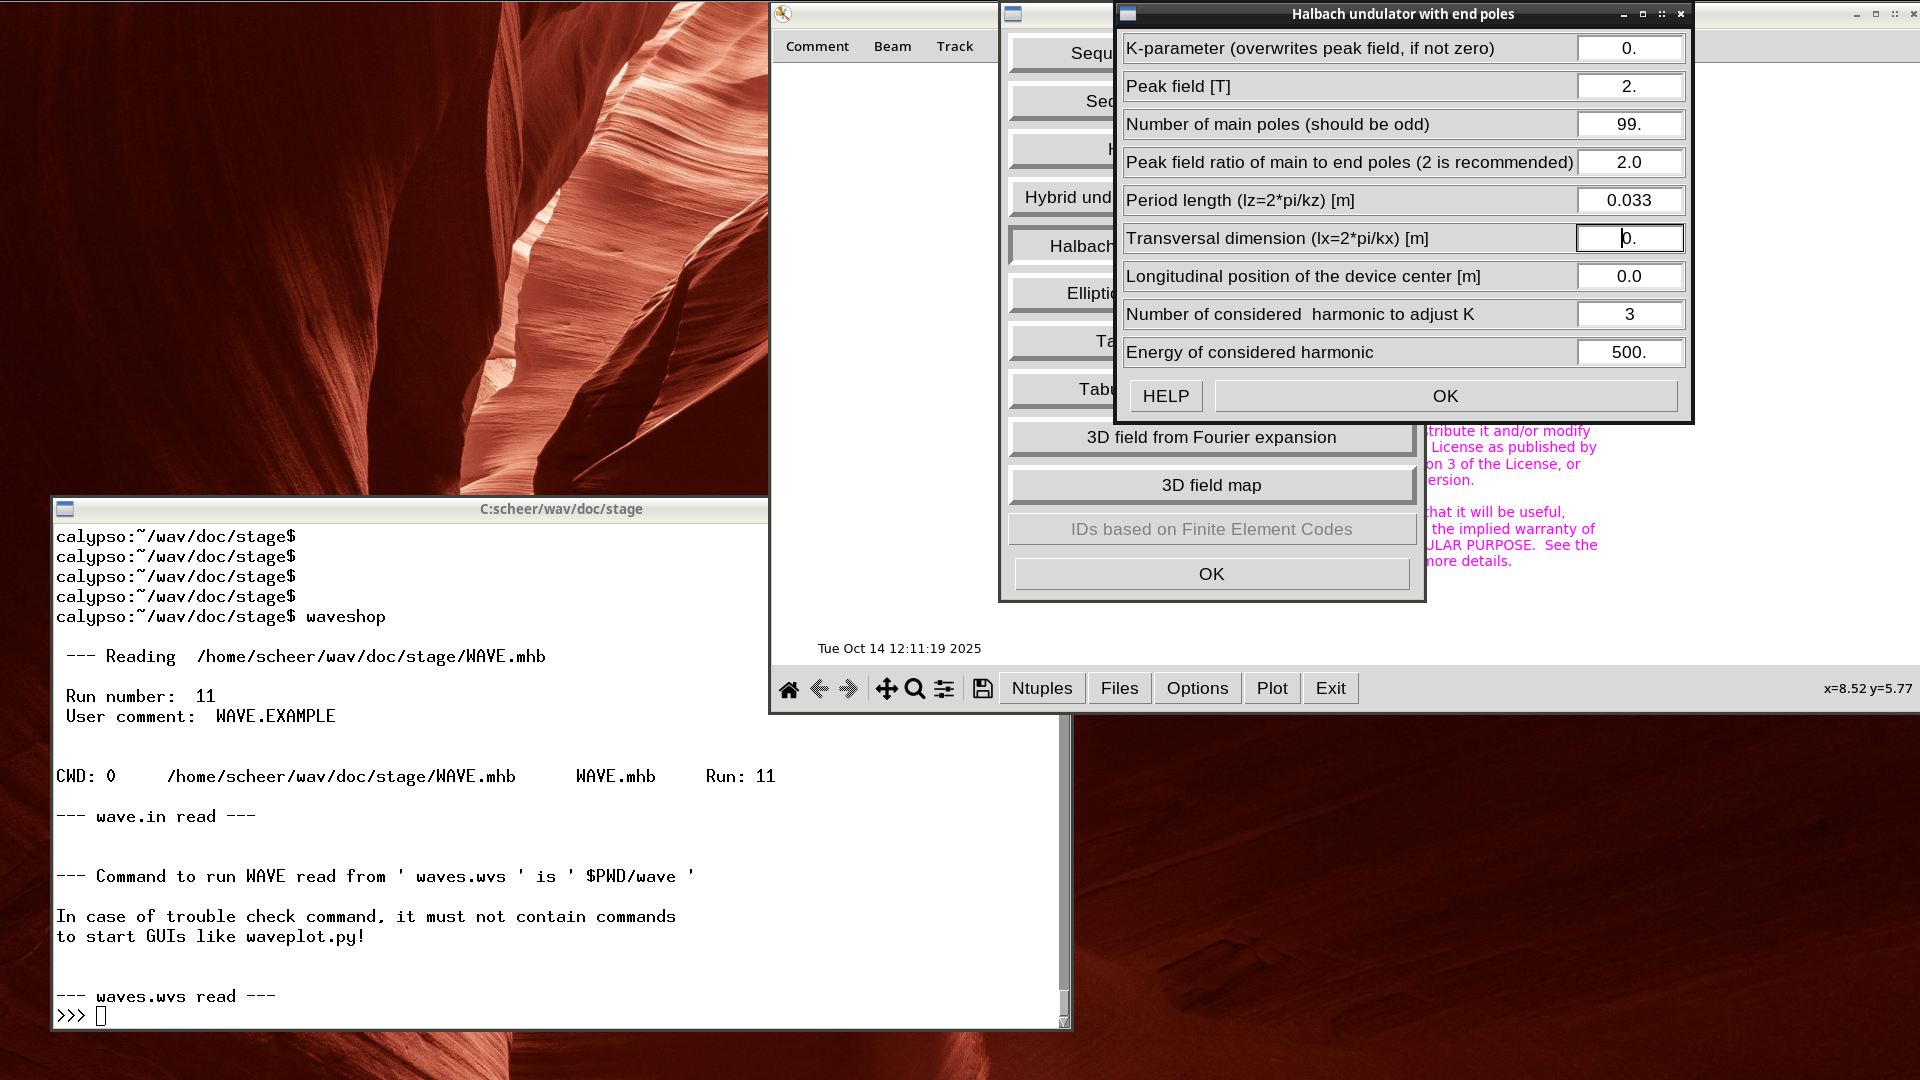
\includegraphics[width=0.6\textwidth]
    {pics/halbasy_undulator.png}
    \caption{Parameters of the undulator}
    \label{ex1fig1}
\end{figure}

Now we set up an undulator model with \gtis{99} main poles and two
endpoles, i.e. a \gtis{50} periods undulator. The period length is
\gtise{0.033m}.
In addition, the third harmonic should be at \gtis{500eV}
(Fig.\ref{ex1fig1}).

\underline{Note:}
\begin{itemize}
\item
\vspace*{-0.5cm} Selecting a harmonic overrides the magnetic field value given in the shown
menu.
\item
For this model, \gtis{z} is the longitudinal
coordinate, while the WAVE coordinate system is such, that \gtis{x} is the
longitudinale axis.
\end{itemize}

We close the last two menus and go back the main input menu.

Next, we adjust the observation pinhole.

\begin{itemize} \renewcommand\labelitemi{--}

\item
Click

\witem{Spectrum calculations}
\witem{Pinhole definition}

and set the pinhole width and height to \gtis{0.002}

\item
Hit \gtis{OK} and choose:

\witem{Spectral range}

Set the lowest and highest photon energies to \gtis{495.0} and
\gtis{505.0} eV, respectively.

\end{itemize}

We run \W by clicking \gtis{Run} in the toolbar.

\begin{figure}[htb]
    \centering
    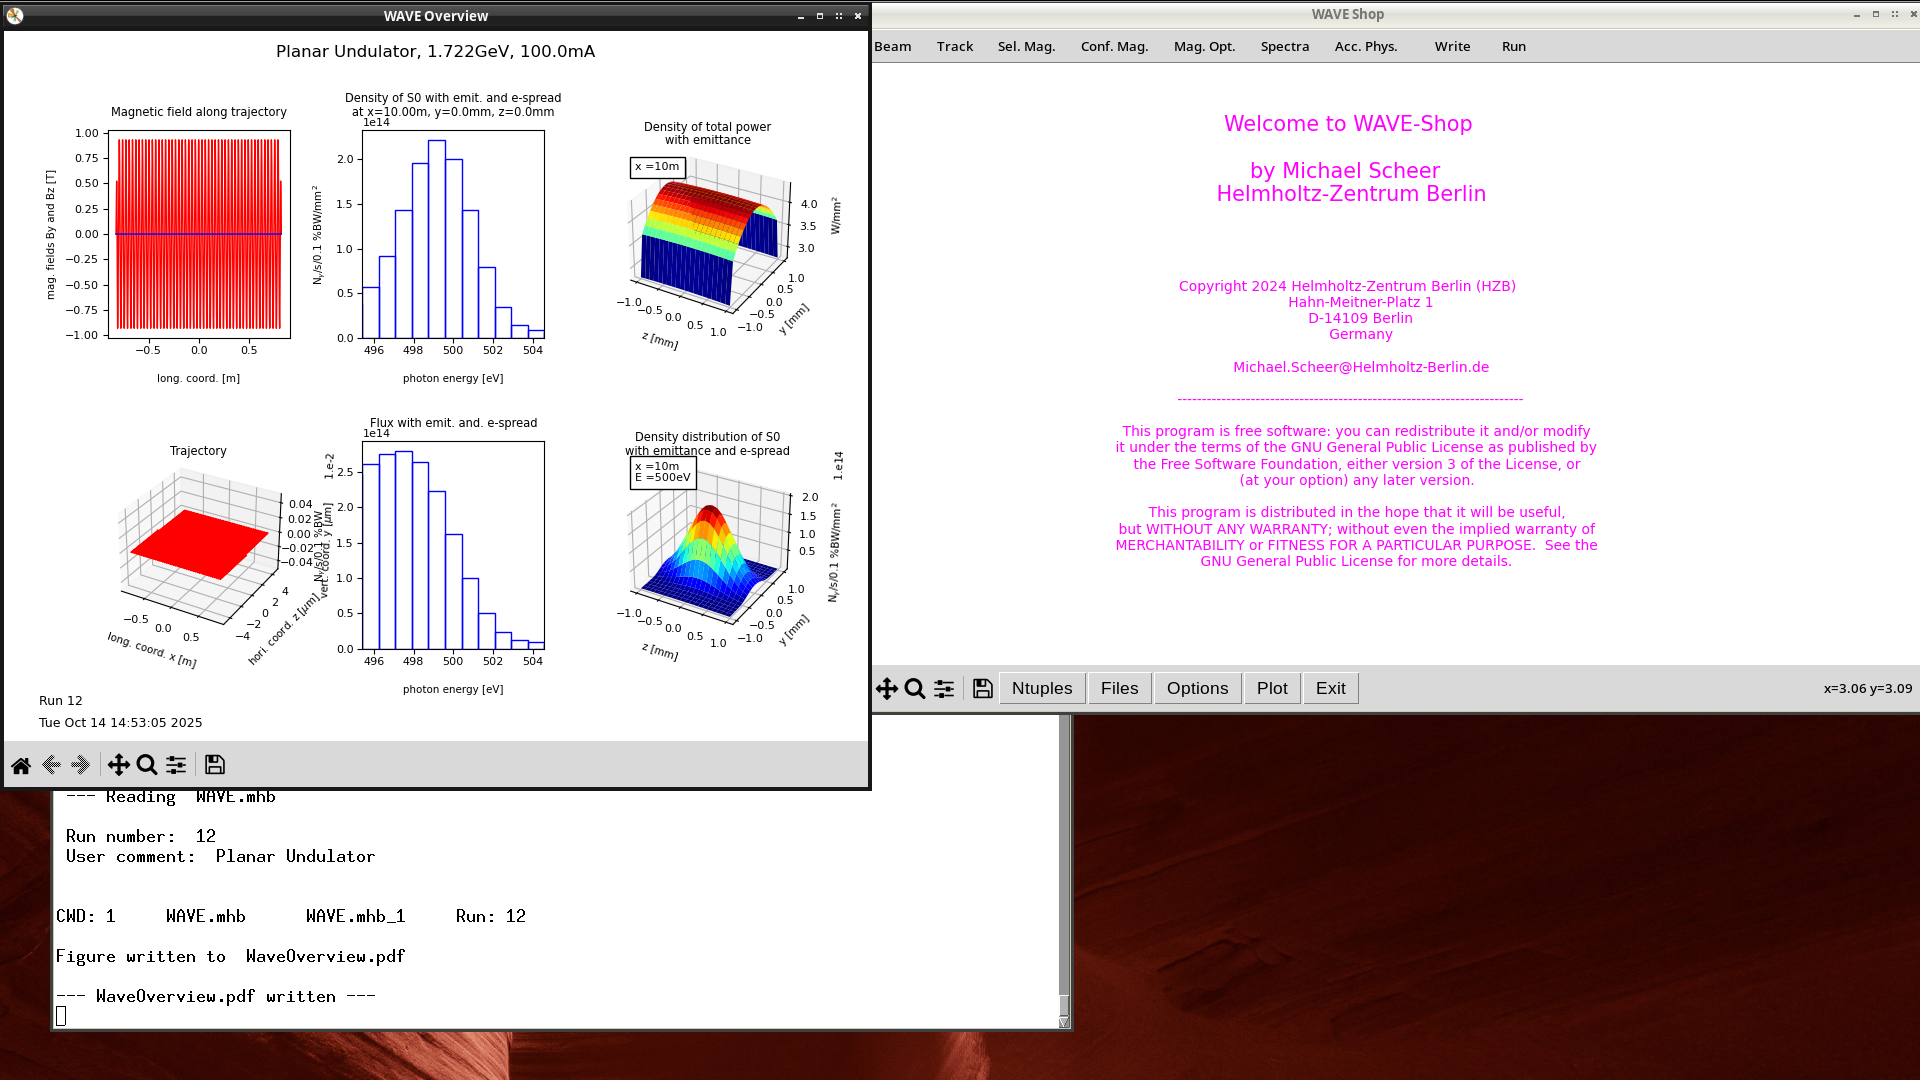
\includegraphics[width=0.9\textwidth]{pics/ex1fig3_overview.png}
    \caption{Overview of plots}
    \label{ex1fig3}
\end{figure}

In the terminal we see some warnings, which can be ignored. They could
be relevant in the case of very precise calculations. To avoid them,
one could increase the number of grid points in the Pinhole menu from 21 to
51, but that slows down everything for nearly no benefit.

Click the button \gtis{Plot}, select \gtis{Overview}, and check the results.

Before we finish this examples, we open the output file \wo~with a
text editor.

\begin{figure}[htb]
    \centering
    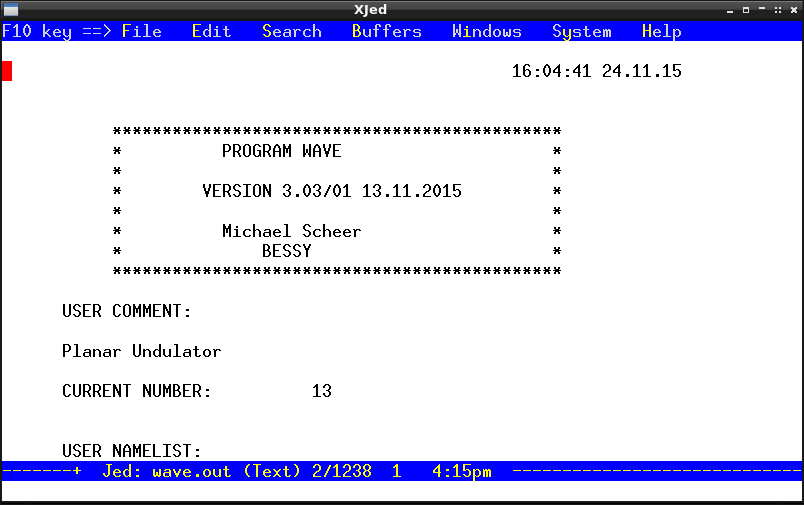
\includegraphics[width=0.9\textwidth]{pics/ex1_wave_out.png}
    \caption{The output file \textit{wave.out}}
    \label{ex1fig2}
\end{figure}

This file contains a summary of the input variables and results of the
calculations, as well as warnings and error messages. At the top you
see your user comment (the variable \scap{CODE} in \wi) and the current
run number, which is stored in the file \scap{WAVE\_CODE.DAT}. The
output file is a good place to check the input parameters of the
magnetic field model, the beam parameters etc..

As a beginner, you
should at least once study the file thorougly, although it might
contain some information you don't understand at this moment{\ldots}

%\newpage
Now it's up to you, to fumble around with the parameters of the
menus described above and watch the effects. In case of trouble, you
can always go back by copying
\gtis{\$WAVE/input/wave\_example\_1.in}
to
\gtis{wave.in}.

Proposed exercise: Compare \wi and \we.
